%This is "sig-alternate.tex" V2.0 May 2012
% This file should be compiled with V2.5 of "sig-alternate.cls" May 2012
%
% This example file demonstrates the use of the 'sig-alternate.cls'
% V2.5 LaTeX2e document class file. It is for those submitting
% articles to ACM Conference Proceedings WHO DO NOT WISH TO
% STRICTLY ADHERE TO THE SIGS (PUBS-BOARD-ENDORSED) STYLE.
% The 'sig-alternate.cls' file will produce a similar-looking,
% albeit, 'tighter' paper resulting in, invariably, fewer pages.
%
% ----------------------------------------------------------------------------------------------------------------
% This .tex file (and associated .cls V2.5) produces:
%       1) The Permission Statement
%       2) The Conference (location) Info information
%       3) The Copyright Line with ACM data
%       4) NO page numbers
%
% as against the acm_proc_article-sp.cls file which
% DOES NOT produce 1) thru' 3) above.
%
% Using 'sig-alternate.cls' you have control, however, from within
% the source .tex file, over both the CopyrightYear
% (defaulted to 200X) and the ACM Copyright Data
% (defaulted to X-XXXXX-XX-X/XX/XX).
% e.g.
% \CopyrightYear{2007} will cause 2007 to appear in the copyright line.
% \crdata{0-12345-67-8/90/12} will cause 0-12345-67-8/90/12 to appear in the copyright line.
%
% ---------------------------------------------------------------------------------------------------------------
% This .tex source is an example which *does* use
% the .bib file (from which the .bbl file % is produced).
% REMEMBER HOWEVER: After having produced the .bbl file,
% and prior to final submission, you *NEED* to 'insert'
% your .bbl file into your source .tex file so as to provide
% ONE 'self-contained' source file.
%
% ================= IF YOU HAVE QUESTIONS =======================
% Questions regarding the SIGS styles, SIGS policies and
% procedures, Conferences etc. should be sent to
% Adrienne Griscti (griscti@acm.org)
%
% Technical questions _only_ to
% Gerald Murray (murray@hq.acm.org)
% ===============================================================
%
% For tracking purposes - this is V2.0 - May 2012

\documentclass{sig-alternate}

\begin{document}
%
% --- Author Metadata here ---
\conferenceinfo{FDG}{2016} % location????El Paso, Texas USA}
\CopyrightYear{2016} % Allows default copyright year (20XX) to be over-ridden - IF NEED BE.
%\crdata{0-12345-67-8/90/01}  % Allows default copyright data (0-89791-88-6/97/05) to be over-ridden - IF NEED BE.
% --- End of Author Metadata ---

\title{Monte Carlo Tree Search with Options\\for General Video Game Playing}
%\subtitle{[Extended Abstract]
%\titlenote{A full version of this paper is available as
%\textit{Author's Guide to Preparing ACM SIG Proceedings Using
%\LaTeX$2_\epsilon$\ and BibTeX} at
%\texttt{www.acm.org/eaddress.htm}}}
%
% You need the command \numberofauthors to handle the 'placement
% and alignment' of the authors beneath the title.
%
% For aesthetic reasons, we recommend 'three authors at a time'
% i.e. three 'name/affiliation blocks' be placed beneath the title.
%
% NOTE: You are NOT restricted in how many 'rows' of
% "name/affiliations" may appear. We just ask that you restrict
% the number of 'columns' to three.
%
% Because of the available 'opening page real-estate'
% we ask you to refrain from putting more than six authors
% (two rows with three columns) beneath the article title.
% More than six makes the first-page appear very cluttered indeed.
%
% Use the \alignauthor commands to handle the names
% and affiliations for an 'aesthetic maximum' of six authors.
% Add names, affiliations, addresses for
% the seventh etc. author(s) as the argument for the
% \additionalauthors command.
% These 'additional authors' will be output/set for you
% without further effort on your part as the last section in
% the body of your article BEFORE References or any Appendices.

\numberofauthors{3} %  in this sample file, there are a *total*
% of EIGHT authors. SIX appear on the 'first-page' (for formatting
% reasons) and the remaining two appear in the \additionalauthors section.
%
\author{
% You can go ahead and credit any number of authors here,
% e.g. one 'row of three' or two rows (consisting of one row of three
% and a second row of one, two or three).
%
% The command \alignauthor (no curly braces needed) should
% precede each author name, affiliation/snail-mail address and
% e-mail address. Additionally, tag each line of
% affiliation/address with \affaddr, and tag the
% e-mail address with \email.
%
% 1st. author
\alignauthor
Maarten de Waard\\
       \affaddr{University of Amsterdam}\\
       \affaddr{Science Park 904}\\
       \affaddr{Amsterdam, The Netherlands}\\
       \email{mrtndwrd@gmail.com}
% 2nd. author
\alignauthor
Diederik M. Roijers\\
       \affaddr{University of Amsterdam}\\
       \affaddr{Science Park 904}\\
       \affaddr{Amsterdam, The Netherlands}\\
       \email{D.M.Roijers@uva.nl}
% 3rd. author
\alignauthor
Sander C.J. Bakkes\\
       \affaddr{University of Amsterdam}\\
       \affaddr{Science Park 904}\\
       \affaddr{Amsterdam, The Netherlands}\\
       \email{S.C.J.Bakkes@uva.nl}
   }% use '\and' if you need 'another row' of author names
% There's nothing stopping you putting the seventh, eighth, etc.
% author on the opening page (as the 'third row') but we ask,
% for aesthetic reasons that you place these 'additional authors'
% in the \additional authors block, viz.
%\additionalauthors{Additional authors: John Smith (The Th{\o}rv{\"a}ld Group,
%email: {\texttt{jsmith@affiliation.org}}) and Julius P.~Kumquat
%(The Kumquat Consortium, email: {\texttt{jpkumquat@consortium.net}}).}
\date{30 July 1999}
% Just remember to make sure that the TOTAL number of authors
% is the number that will appear on the first page PLUS the
% number that will appear in the \additionalauthors section.

\maketitle
\begin{abstract}
ABSTRACT
\end{abstract}

% A category with the (minimum) three required fields
%\category{H.4}{Information Systems Applications}{Miscellaneous}
%A category including the fourth, optional field follows...
%\category{D.2.8}{Software Engineering}{Metrics}[complexity measures, performance measures]

%\terms{Theory}

\keywords{MCTS, GVGAI, General Game AI, Options}

\chapter{Introduction}
\label{sec:introduction}
% This might be useful for AAMAS or something, but not for gaming comferences
%
%In the history of AI algorithms, playing games has been one of the objectives
%for a long time. These algorithms typically maximize their score or win
%probability. Early AI algorithms focused on simple games like tic tac toe,
%later focus was shifted to chess and even later to Go. Nowadays, many
%algorithms are designed for solving computer games. For example a lot of
%strategy games offer computer controlled contestants. 

General video game playing is a challenging problem, and since many real-world
problems can be modelled as a game, AI algorithms that can play
complex games successfully are often highly effective problem solvers as well.
%Game-specific AIs work well, but it is a time consuming task to create an AI for every game.  
Therefore, recent research focusses on algorithms capable of
solving several games with differing types of objectives.  A very common general
game solving approach is to use a tree search in order to select the best action
in a game state. The tree search is repeated in every new state until the game
ends. A popular example of this is \emph{Monte Carlo Tree Search (MCTS)}, which
achieves reasonable results on many games.

However, since many games are too complex to plan far ahead in a reasonable
time frame, planning by tree search based methods often only considers short-term
score differences and does not incorporate long-term plans. Moreover, many
algorithms lack common video game knowledge and do not use any of the knowledge
gained from the previous games.

In contrast, when humans play a game we expect them to do assumptions about
its mechanics, e.g., pressing the left button often results in the player's
avatar moving to the left on the screen. Players can use these assumptions to
learn how to play the game more quickly. Furthermore, human players have an
abstraction layer over their action choices; instead of choosing one action at a
time they define a specific subgoal for themselves.  For example: when there is
a portal on screen, a human player is likely to try to find out what the portal
does by walking towards it. Walking towards the portal can then be seen as a
subgoal of playing the game.

%\todo{Introduction of options (abstract thinking level)}
%	\todo{Introduction of learning about options}
%	\todo{Options have never been used with MCTS, this combination is
%	revolutionary!}

In certain situations, it is clear how such a subgoal can be achieved and a
sequence of actions, or \emph{policy}, can be defined to achieve it. A policy to
achieve a subgoal is called an option. Thus, an option selects an action, given
a game state, that aims at satisfying its subgoal.  Options, in this context, are
game-independent. For example, an option that has reaching a specific location
in the game (for example a portal) as its objective, selects actions using a
path planning heuristic that will reach the goal location. In this paper a new
algorithm, called \emph{Option MCTS (O-MCTS)} is introduced that extends MCTS to
use options. Because O-MCTS chooses between options rather than actions when
playing a game, we expect it to be able to plan at a higher level of
abstraction. Over time, information can be learned about the type of options
that is more useful in a game, which can be used to focus exploration of the
search tree to promising options. This information can also be transferred in
order to increase performance on a next, possibly harder, level. 

The algorithm will be benchmarked on four sets of games from the General Video
Game AI Competition \cite{perez2014}, against the standard Monte Carlo Tree
Search algorithm that is provided by that competition.  Our results indicate
that the resulting algorithm outperforms traditional MCTS.



\chapter{Background}
\label{sec:background}

This chapter explains the most important concepts needed to understand the
algorithms that are proposed in this thesis. The first section describes
\emph{Markov decision processes (MDPs)}, a formalization of the type of problem
that the algorithms have to solve. The next section describes MCTS, a tree
search algorithm that is commonly used on games and other MDPs. Subsequently,
options will be formalized, these simulate the idea of defining subgoals and
how to reach them. Then, the basics of Q-learning are described, from which SMDP
Q-learning is derived. Finally the \emph{video game description language (VGDL)}
is explained. This is the protocol that is used by the GVGAI competition to
generate the many different games the competition offers, that all use the same
interaction framework with the game playing algorithms.

\section{Markov Decision Processes}
\label{subsec:mdps}
In this thesis, games will be treated as MDPs, which provide a mathematical
framework for use in decision making problems. An MDP is formally defined as a
tuple $\langle S, A, T, R \rangle$, where $S$ denotes the set of states. Since an MDP
is fully observable, a state contains all the information of the
game's current condition: locations of sprites like monsters and portals; the
location, direction and speed of the avatar; which resources the avatar has
picked up; etcetera. $A$ is a finite set of actions, the input an agent can
deliver to the game. $T$ is a transition function defined as $T : S \times A
\times S \rightarrow \left[0,1\right]$. It specifies the probabilities over the
possible next states, when taking an action in a state.  $R$ is a reward
function defined as $R: S \times A \times S \rightarrow \mathbb{R}$. In this
case, when the game score changes, the difference is viewed as the reward.
Algorithms typically maximize the cumulative reward, which is analogous to the
score. An MDP by definition has the \emph{Markov property}, which means that the
conditional probability distribution of future states depends only upon the
present state. No information from previous states is needed. Algorithms do not
have access to $T$ and $R$ in the scope of this thesis.

For example, for the game Zelda, a state $s$ consists of the location, rotation
and speed of the avatar and the location of the avatar's sword, the monsters, the
walls and the key and portal that need to be found. $S$ is the set of all
possible states, so all possible combinations of these variables. The action set
$A$ consists of the actions \textsc{up}, \textsc{down}, \textsc{left},
\textsc{right} and \textsc{use}, the latter of which spawns the sword in front
of the avatar for a couple of time steps. The transition function $T$ defines the
transition from a state, given an action.  This means that the transition
defines the change in location of the monsters and the avatar and if any of the
sprites disappear (e.g. when the avatar picks up the key). Note that, since
the transition function is not by definition deterministic, the resulting state
from an action $a$ in state $s$ is not always the same state. For instance,
because a monster moves about randomly, it could have moved left or right in the
new state. The reward function describes the change in game score, given a
state, action and resulting next state, for example when the avatar kills a
monster with the action \textsc{use}, its score will increase with 1.

\section{Monte Carlo Tree Search}
\label{subsec:mcts}
Monte Carlo methods have their roots in statistical physics, where they have
been used to approximate intractable integrals. Abrahamson
\cite{abramson1990expected} demonstrated theoretically that this sampling method
might be useful for action selection in games as well.  In 2001, Monte Carlo
methods were effectively used for bridge \cite{ginsberg2001gib}. The real
success of MCTS started in 2006, when the tree search method and UCT formula
were introduced, yielding very good results in Computer Go
\cite{gelly2006modification}. Since 2006, the algorithm has been extended with
many variations and is still being used for other (computer) games
\cite{browne2012survey}, including the GVGAI competition
\cite{perez2014knowledge}.

\begin{figure}
	\centering
	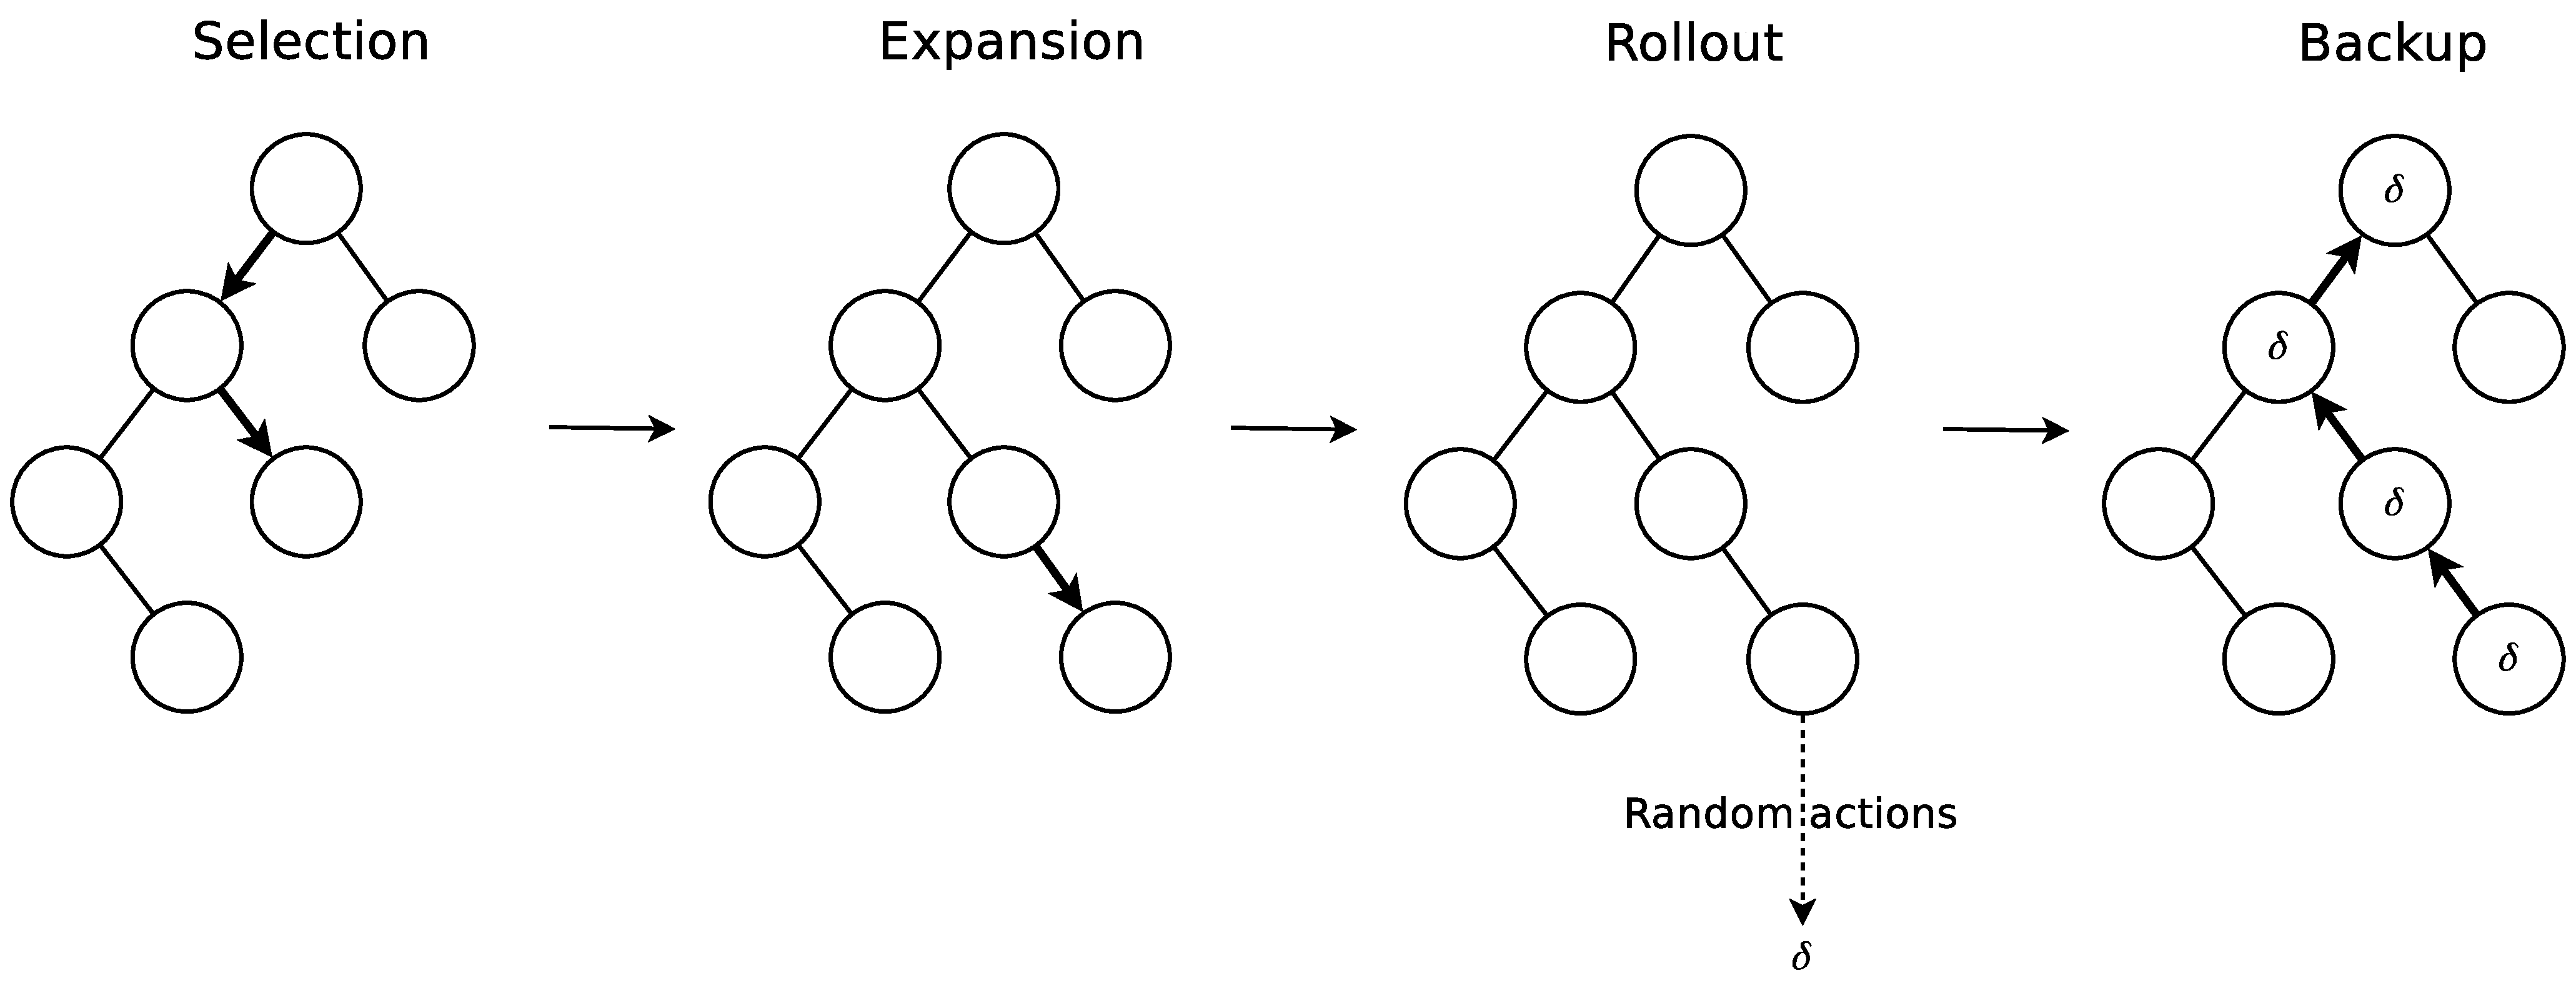
\epsfig{file=includes/mcts-wide.eps, width=\textwidth}
	\caption{One Monte Carlo tree search iteration}
	\label{fig:mcts}
\end{figure}

This section explains how MCTS approximates action values for states.  A tree is
built incrementally from the states and actions that are visited in a game. Each
node in the tree represents a state and each connection in the tree represents
an action taken in that state leading to a new state, which is represented by
the next tree node.  The process, as explained in Figure \ref{fig:mcts},
consists of four phases that are constantly repeated. It is started with the
current game state, which is represented by the root node of the tree. The first
action is chosen by an \emph{expansion strategy} and subsequently simulated,
resulting in a new game state, for which a new node is created. After expansion,
a \emph{rollout} is done from the new node, which means that a simulation is run
from the new node applying random actions until a predefined stop criterion is
met or the game ends. Finally, the score difference resulting from the rollout
is \emph{backed up} to the root node, which means that the reward is saved to the
visited nodes.  Then a new iteration starts. When all actions are expanded in a
node, that node is deemed \emph{fully expanded} and uses a \emph{selection
strategy} to select a next node. When a node is selected that is not fully
expanded, the expansion strategy is used to create a new node, after which a
rollout takes place and the results are backed up thereafter.

The selection strategy selects optimal actions in internal tree nodes, by
analyzing the values of their child nodes. An effective and very popular
selection strategy is the \emph{upper confidence tree (UCT)}
\cite{kocsis2006bandit}, which balances the choice between poorly explored
actions with a high uncertainty about their value and actions that have been
explored extensively, but have a higher value. A child node $j$ is selected to
maximize
\begin{equation}
	\label{eq:uct}
	UCT = v_{s'} C_p \sqrt{\frac{2 \ln n_s}{n_{s'}}}
\end{equation}
Where $v_{s'}$ is the value of child $s'$ as calculated by the backup function,
$n_s$ is the number of times the current node $s$ has been visited, $n_{s'}$ is
the number of times child $s'$ has been visited and $C_p > 0$ is a constant,
often set to $\sqrt{2}$, that shifts priority from exploration to exploitation.

The traditional expansion strategy is to explore each action at least once in
each node. After all actions have been expanded, the node applies the selection
strategy for further exploration. Some variants of MCTS reduce the branching
factor of the tree by only expanding the nodes selected by a special expansion
strategy. A specific example is the \emph{crazy stone} algorithm
\cite{coulom2007efficient}, which is an expansion strategy that was designed
specifically for Go. We will use an adaptation of this strategy in the algorithm
proposed in Chapter \ref{sec:learning}.  When using crazy stone, an action $i$
is selected with a probability proportional to $u_i$
\begin{equation}
	\label{eq:crazystone}
	u_i = \exp\left(K \frac{\mu_0 - \mu_i}{\sqrt{2\left(\sigma_0^2 +
\sigma_i^2\right)}}\right) + \epsilon_i
\end{equation}
Each action has an estimated value $\mu_i$ ordered in such a way that $\mu_0 >
\mu_1 > \ldots > \mu_N$, and a variance $\sigma_i^2$. $\epsilon_i$ prevents 
the probability of selecting a move to reach zero and its value is proportional to
the ordering of the expected values of the possible actions. K is a constant
that influences the exploration/exploitation trade off.
\begin{equation}
	\label{eq:epsilon}
	\epsilon_i = \frac{0.1 + 2^{-i} + a_i}{N}
\end{equation}
Where $a_i$ is 1 when an action is \emph{an atari move}, a go-specific
move that can otherwise easily be underestimated by MCTS, and otherwise 0.

After a rollout, the reward is backed up, which means that the estimated value
for every node that has been visited in this iteration is updated with the
reward of this simulation. Usually the estimated value of a node is the average
of all rewards backed up to that node.

\section{Q-learning}
\label{subsec:qlearning}
Q-learning is a relatively simple model free temporal difference learning method
that was proposed in 1992 \cite{watkins1992q}. The \emph{Q-value} of an action
for a state, $Q(s, a)$, is the discounted reward that can be achieved by
applying action $a$ to state $s$ and following the optimal policy afterwards. By
learning Q-values for every action in every state, it can estimate an optimal
policy. 

The general idea of Q-learning is to incrementally save the reward from the MDP,
in combination with the current Q-value of the state-action pair: the update
function uses the reward and the maximum of the Q-values of the next state. By
always using the maximum value of the next state as well, the Q-value function
will eventually converge to a depiction of the maximum future reward for a
state-action pair. More specifically, the update function for a state-action
pair is
\begin{equation}
	\label{eq:qlearning}
	Q(s, a) \gets Q(s, a) + \alpha \left(r + \gamma \max_{a \in A} Q(s', a) - Q(s, a)\right),
\end{equation}
where $r$ is the reward that is achieved by using action $a$ in state $s$,
leading to state $s'$. The algorithm has two parameters: $\gamma$ is the
discount factor, which indicates the importance of future states. $\alpha$ is the
learning rate, which determines how quickly the Q-values are updated.
Q-learning is shown to converge, even in problems with a stochastic transition
function, if $\alpha$, $\alpha$ decreases over time. In practice, however, it is
often set to $0.1$. The Q-table can be used to find the optimal policy by, for
each state $s$, selecting the action $a$ that maximizes $Q(s, a)$. Because after
each action only one state-action pair is being updated, Q-learning can take a
long time to converge, but it is guaranteed to converge to the optimal policy,
given that during exploration, each state-action pair is visited an infinite
number of times.

\section{Options}
\label{subsec:options}
In order to mimic human game playing strategies, defining subgoals and subtask,
we use options. Options have been proposed by Sutton et al.
\cite{sutton1999between} as a method to incorporate temporal abstraction in
field of reinforcement learning. A lot of progress has been made since, but a
lot of the research seems to focus on learning algorithms and little work is
done on combining options with tree search methods \cite{barto2003recent}, which
offer a model free planning framework.

An option is a predefined method of reaching a specific subgoal. Formally, it is
a triple $\langle I, \pi, \beta\rangle$ in which $I \subseteq S$ is an
initiation set, $\pi: S \times A \rightarrow [0, 1]$ is a policy and $\beta: S^+
\rightarrow[0,1]$ is a termination condition.  A policy $\pi$ defines the action
that should be taken in a state. The initiation set $I$ is a set of states in
which the option can be started. Typically, when the option starts, policy $\pi$
will be followed, until a state is reached that satisfies a termination
condition in $\beta$. After that, a new option is chosen and followed. 

Using options in an MDP removes the Markov property for that process: the state
information alone is no longer enough to predict an agent's actions, since the
actions are now not only state-dependant, but dependant on what option the agent
has chosen in the past as well. According to \cite{sutton1999between}, we can
now view the process as a \emph{semi-Markov decision process (SMDP)}
\cite{duff1995reinforcement}, where options are viewed as actions of variable
length. In this thesis, we will keep calling the original action set of the MDP
$A$, and the set of options $O$.  Normal actions can be treated as options as
well.  An option for action $a \in A$ has a initiation set $I = S$, the policy
$\pi$ is taking action $a$ in all the states.  The termination condition $\beta$
is that action $a$ should be performed once.


\section{Video Game Description Language}
\label{subsec:vgdl}
In order to test algorithms on several different games, a framework is used that
can access a large number of games in a similar manner. The GVGAI competition
uses the \emph{video game description language (VGDL)} \cite{schaul2013video},
in which games can be defined easily. VGDL aims to be a description language
for games that is clear, human readable and unambiguous. Games are easy to parse
and it is possible to automatically generate them. Using a VGDL framework,
algorithms can access all the games in a similar manner, resulting in a fair
method to compare their performances on several games.

To define a game in VGDL, two files are required. Firstly, the game description
should be made, which defines for each type of object what character in the
level description it corresponds to, what it looks like in a game visualization,
how it interacts with the rest of the game, and when it disappears from the
game. Secondly, a level description file is needed, in which each character maps
to an object in the game. The location in the file corresponds to its grid
location in the game. By defining these two files, a wide spectrum of games
can be created. A more extensive explanation of VGDL can be found in Chapter
\ref{subsec:games}.

In this thesis, we will use a Java implementation made for the GVGAI
competition, which comes with many games. In this version, algorithms only
observe the game information: score, game tick (timestep), the set of possible
actions and information about if the game is over and if the player won; Avatar
information: its position, orientation, speed and resources; and screen
information: Which sprites are on what location of the screen, and the size (in
pixels) of the game grid's blocks.

The algorithm proposed in this thesis will be
benchmarked on these games, using the rules of the GVGAI competition. 
This means that the algorithms do not have any access to the game and level
descriptions. When an algorithms starts playing a game, it typically knows
nothing of the game, except for the observation described above.


\section{Planning}
\label{sec:planning}

%\todo{hieronder: Dit is onze contributie, ``a novel algorithm'', ``key
%insight'', ``main objective''}
%\todo{Wat gaan we doen: herhalen main objective, teruggrijpen op background en
%introductie}

Planning over options is traditionally done by applying Q-learning to a set of
options instead of the set of actions \cite{sutton1999between}. Q-learning
learns the transition and reward for each state, but as game complexity
increases, the state space grows as well, increasing Q-learning's memory usage
and computation time immensely. In this section we introduce \emph{option Monte
Carlo tree search (O-MCTS)}, a novel algorithm that plans over options using
MCTS, enabling the use of options in complex MDPs.  The resulting algorithm
achieves higher scores on complex games that have several sub-goals than
traditional MCTS.

%\todo{How to combine options with MCTS - what problems (challenges) occur?}
In normal MCTS, an action is represented by a connection from a state to a next
state. An option spans over several actions, which influences the tree search
method. Furthermore, when many options are defined, the branching factor of the
algorithm increases significantly. This problem will be addressed in the next
section, where we will incorporate learning in the algorithm.

\begin{figure}
	\centering
	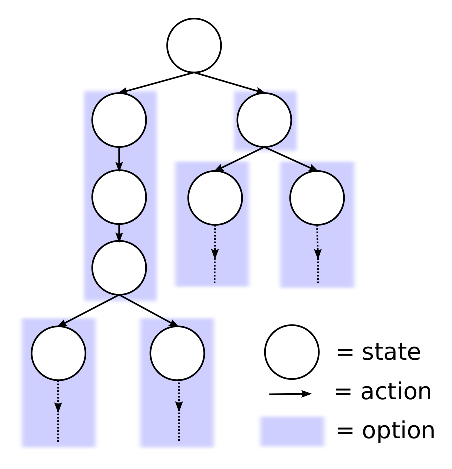
\epsfig{file=includes/omcts.eps, width=.5\columnwidth}
	\caption{The search tree constructed by O-MCTS. In each blue box, one option
	is followed. The arrows represent actions chosen by the option. An arrow
leading to a blue box is an action chosen by the option represented by that box.}
	\label{fig:omcts-tree}
\end{figure}

Traditionally, when a node is at depth $n$, we know that $n$ actions have been
chosen to arrive at that node and the time in that node is $t+n$. If nodes in
O-MCTS would represent options and connections would represent option selection,
this property would be lost, complicating the comparison of different nodes at
the same level in the tree. Therefore, we chose to keep the tree representation
the same: a node represents a state, a connection represents an action. We
introduce a change in the expansion and selection strategies, which select
options, rather than actions. When a node has an unfinished option, the next
node will be created using an action selected by that option. When a node
contains a finished option (meaning that the current state satisfies its
termination condition $\beta$), a new option can be chosen by the expansion or
selection strategy. The search tree now looks like Figure \ref{fig:omcts-tree},
in which each blue box represents one option.

Options are hand defined. We created a set of options most of which use the A
Star algorithm to navigate the agent towards a specific game sprite or location
\cn.

\begin{algorithm}
	\caption{$\mathsf{O-MCTS}(O, r, t, d)$}
	\label{alg:omcts}
	\begin{algorithmic}[1]
		\State $C_{s \in S} \gets \emptyset$ \Comment{$\mathbf{c}_s$ is the set of children nodes of $s$}
		\State $\mathbf{o} \gets \emptyset$ \Comment{$o_s$ will hold the option followed in $s$}
		\While {$time\_taken < t$} \label{alg:omcts:mainloop}
			\State $s \gets r$ \Comment{start from root node}
			\While {$\neg \mathsf{stop}(s, d)$} \label{alg:omcts:innerloop}
				\If{$s \in \beta(o_s)$} \label{alg:omcts:sp} \Comment{if option stops in state $s$}
					\State $\mathbf{p}_s \gets \cup_o (s \in I_{o \in O})$ \Comment{$\mathbf{p}_s$ is available options}
				\Else
					\State $\mathbf{p}_s \gets \{o_s\}$ \Comment{no new option can be selected}
				\EndIf \label{alg:omcts:ep}
				\State $\mathbf{m} \gets \cup_o (o_{s \in \mathbf{c}_s})$ \Comment{set $\mathbf{m}$ to expanded options}
				\If{$\mathbf{p}_s = \mathbf{m}$} \Comment{if all options are expanded}
					\State $s' \gets \max_{c \in \mathbf{c}_s} \mathsf{uct}(s, c)$ \label{alg:omcts:uct} 
						\Comment{child from eq. \ref{eq:uct}}
					\State $s \gets s'$ \label{alg:omcts:ss} 
						\Comment{continue loop with new node $s'$}
				\Else \label{alg:omcts:sexpand}
					\State $\omega \gets \mathsf{random\_element}(\mathbf{p}_s - \mathbf{m})$ 
					\State $a \gets \mathsf{get\_action}(\omega, s)$ 
					\State $s' \gets \mathsf{expand}(s, a)$ 
						\Comment{create child $s'$ using $a$}
						\State $\mathbf{c}_s \gets \mathbf{c}_s \cup \{s'\}$ \Comment{add $s'$ to $\mathbf{c}_s$}
					\State $o_{s'} \gets \omega$
					\State \textbf{break} \label{alg:omcts:break}
				\EndIf \label{alg:omcts:eexpand}
			\EndWhile
			\State $\delta \gets \mathsf{rollout}(s')$ \label{alg:omcts:rollout}
				\Comment{simulate until $\mathsf{stop}$}
			\State $\mathsf{back\_up}(s', \delta)$ \label{alg:omcts:backup}
				\Comment{save reward to parent nodes}
		\EndWhile
		\State \Return{$\mathsf{get\_action}(\max_{o \in c_r} \mathsf{value}(o), r)$}
	\end{algorithmic}
\end{algorithm}
\begin{figure}
	\centering
	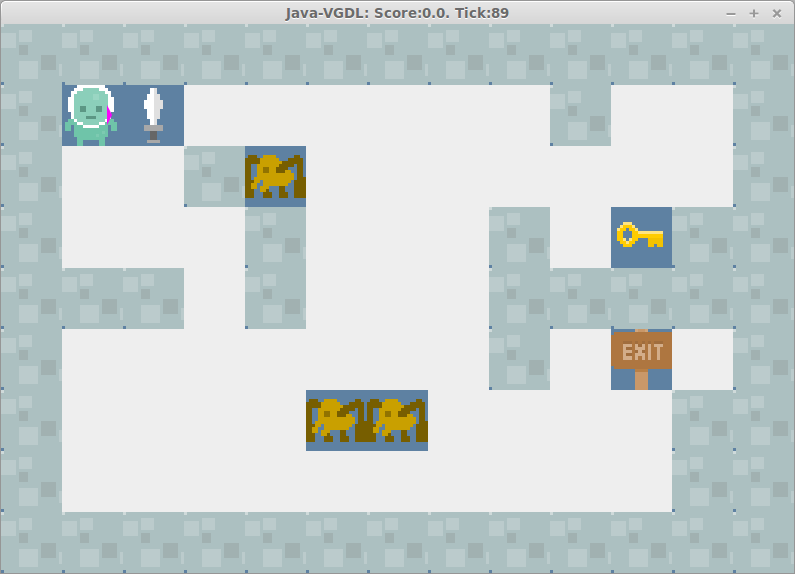
\includegraphics[width=\columnwidth]{includes/zelda}
	\caption{Visual representation of the game Zelda.}
	\label{fig:zelda}
\end{figure}


We describe O-MCTS in Algorithm \ref{alg:omcts}. It is invoked with a set of
options $O$, a root node $r$, a maximum runtime $t$ in milliseconds and a
maximum search depth $d$. Two variables are instantiated. $C_s$ is a set of
sets, containing the set of child nodes for each node and $\mathbf{o}$ contains
which option is followed for each node. The main loop starts at line
\ref{alg:omcts:mainloop}, which keeps the algorithm running until time runs out.
The inner loop runs until a node $s$ is reached that meets a stop criterion
defined by the function \textsf{stop}, or a node is expanded into a new node.
In lines \ref{alg:omcts:sp} until \ref{alg:omcts:ep}, $\mathbf{p}_s$ is set to
all options that are available in $s$. If an option has not finished,
$\mathbf{p}_s$ contains only the current option. Otherwise, it contains all the options $o$ that have state $s$ in their
initiation set $I_o$. For example, when the agent is playing Zelda (see figure
\ref{fig:zelda} and the current
state $s$ shows no NPCs on screen. If there is an option $o$ that goes to NPCs,
$I_o$ will not contain state $s$, because there are no NPCs on screen, rendering
$o$ useless in state $s$. $\mathbf{p}_s$ will thus not contain option $o$, since
$s$ is not in $o$'s initiation set $I_o$.

Then, the four phases of Figure \ref{fig:mcts} are implemented as follows.  If
the set $\mathbf{p}_s$ is the same as the set of options in the children of $s$,
$m$, i.e. all options have been explored at least once in node $s$, a new node
$s'$ is \emph{selected} by \textsf{uct} In line \ref{alg:omcts:ss}, $s$ is
instantiated with the new node $s'$, continuing the inner loop using this node.
If some options are unexplored in node $s$, it is \emph{expanded} with a random,
currently unexplored option by lines \ref{alg:omcts:sexpand} to
\ref{alg:omcts:eexpand}. After expansion or when the stop criterion is reached,
the tree selection loop is stopped and a \emph{rollout} is done, resulting in
score difference $\delta$. This score difference is \emph{backed up} to the
parent nodes of $s$ using the backup function, after which the tree traversal
restarts with the root node $r$.

A couple of functions are used by Algorithm \ref{alg:omcts}. The function
\textsf{stop} returns true when either the game ends in state $s$ or the maximum
depth is reached in $s$. The function \textsf{get\_action} lets option $o$
choose the best action for the state in node $s$, \textsf{apply\_action} applies
the action to state $s$ in the simulator, returning the resulting state.The
function \textsf{expand} creates a new child node for node $s$ with option $o$.
The \textsf{rollout} function chooses random actions until \textsf{stop} returns
true, after which the difference in score achieved by the rollout is returned.
The \textsf{back\_up} function traverses the tree through all parents of $s$,
updating their expected value.

When the time is up, the algorithm chooses an option from $c_r$ corresponding to
the child node with the highest expected value. This option chooses the best
action for the state in the root node and that action is returned. The agent
plays out this action, and runs the algorithm again in the next state it
receives, by creating a new root node $r$ for that state. 

Note that there is a difference between planning using the forward model and
actually acting on the game. During planning, O-MCTS executes options until they are
finished, whereas when a game action has to be chosen, O-MCTS always selects the
option that maximizes the future reward in that state, even if the option chosen
in the previous state was not finished in the current state. This way, when a
state is reached that was not anticipated upon during planning, the right option
will still be chosen.


\section{Learning}
\label{sec:learning}
In order to improve on the O-MCTS planning algorithm, we can estimate
\emph{option values}, the mean and variance of the expected return of an option.
The return $R_o$ for using option $o$ from timestep $t$ to $t+n$ is calculated
by adding the discounted rewards $r_t$ for all of the states visited by that
option.  $$R_o = r_{t} + \gamma r_{t+1} + \gamma^2 r_{t+2} + \cdots + \gamma^n
r_{t+n},$$ where $\gamma \in [0, 1]$ is the discount rate parameter, which
influences the importance of rewards that lay further in the future: an option
with reward 1 at timestep $t$ will get a greater return than an option with the
same reward at timestep $t+1$.  For each type of option the mean and variance of
its discounted reward is kept.  Each time an option is finished, these values
are updated.  By taking the mean of all the option returns a mean option return,
or option value, $\mu_o$ can simply be calculated. We can also calculate the
variance $\sigma_o$ for each option.

\begin{algorithm}
	\caption{$\mathsf{OL-MCTS}(r, max\_time, M)$}
	\label{alg:olmcts}
	\begin{algorithmic}[1]
		\While {$time\_taken < max\_time$} \label{alg:olmcts:mainloop}
			\State $s \gets r$
			\While {$\neg \mathsf{stop}(s)$} \label{alg:olmcts:innerloop}
				\If{$s \in \beta_o$} \label{alg:olmcts:sp}
				\State $\mathsf{updateValues}(\mu_o, s)$
					\State $P_s \gets \cup_o ( s \in I_o)$
				\Else
					\State $P_s \gets \{o\}$ %\Comment{No new option can be selected}
				\EndIf \label{alg:olmcts:scs}
				\If{$n_s < M$}
					% TODO: \mu is eigenlijk niet netjes omdat ik een
					% hoofdletter zou willen gebruiken
					\State $s' \gets \mathsf{crazyStone}(s, \mu)$ \label{alg:olmcts:crazystone}
				\Else
					\State $s' \gets \mathsf{uct}(s)$ \label{alg:olmcts:uct}
				\EndIf \label{alg:olmcts:ecs}
				\State $s \gets s'$ \label{alg:olmcts:ss}
			\EndWhile
			\State $\delta \gets \mathsf{rollout}(s')$ \label{alg:olmcts:rollout}
			\State $\mathsf{back\_up}(s', \delta)$ \label{alg:olmcts:backup}
		\EndWhile
	\end{algorithmic}
\end{algorithm}

Now we have an option value and variance we can use the crazy stone algorithm
to reduce calculation time by shifting the focus of the exploration to promising
options. This means that not all children of a node will be expanded, but only
the ones selected by crazy stone. The algorithm then changes to algorithm
\ref{alg:olmcts}. Most of it is the same, with the exception that crazy stone
selects what node to expand in the first $M$ node visits. Because crazy stone
can select the same option several times, this prevents the algorithm from
expanding all the children, which saves time. 

Crazy stone uses the mean return $R_o$ of each option as its estimated value
$\mu$ for selecting which option to select or expand. After a predefined number
of visits $M$ to a node, the selection strategy $\mathsf{uct}$ is followed to
tweak the option selection.




\section{Experiments}
\label{sec:experiments}
\begin{figure*}
\centering
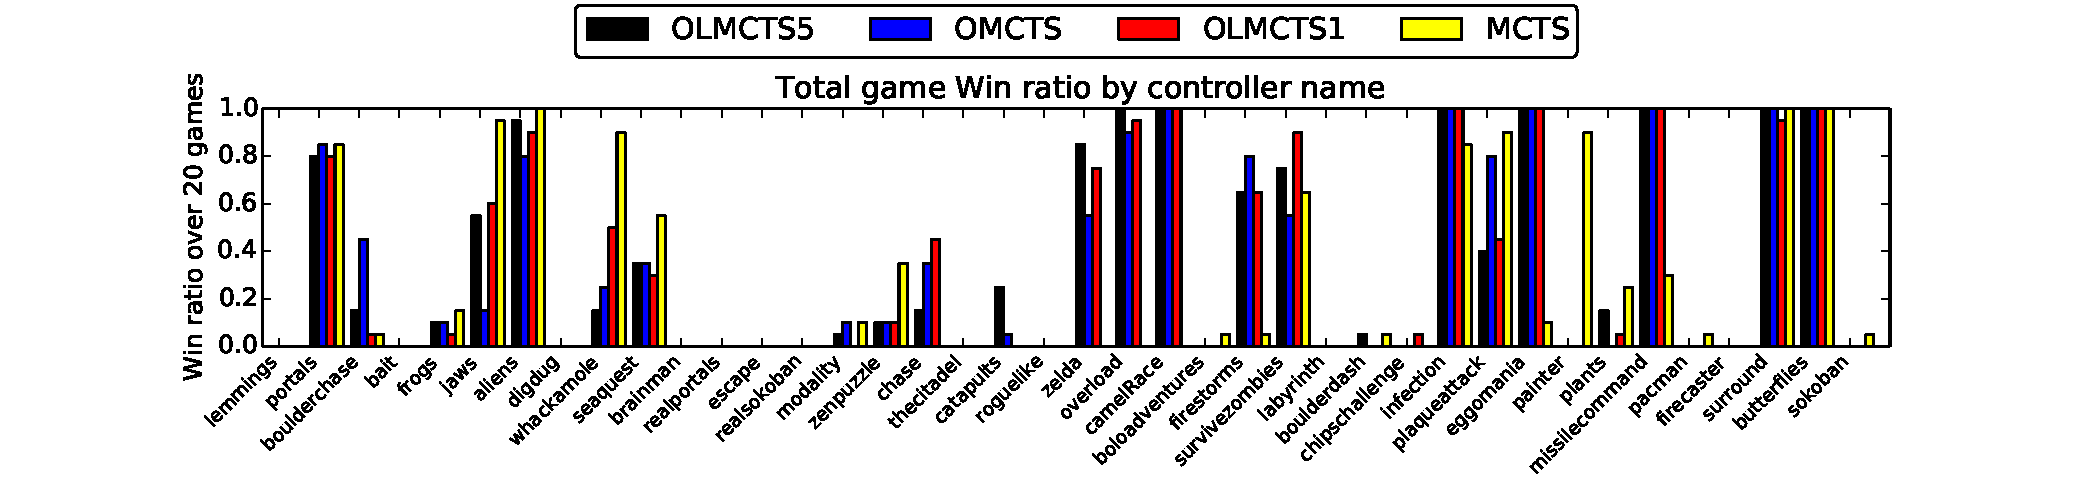
\includegraphics[width=\textwidth]{includes/wins}
%\vspace{-.4cm}
%\caption{Win ratio of the algorithms per game on all levels.}
%\label{fig:wins}
\centering
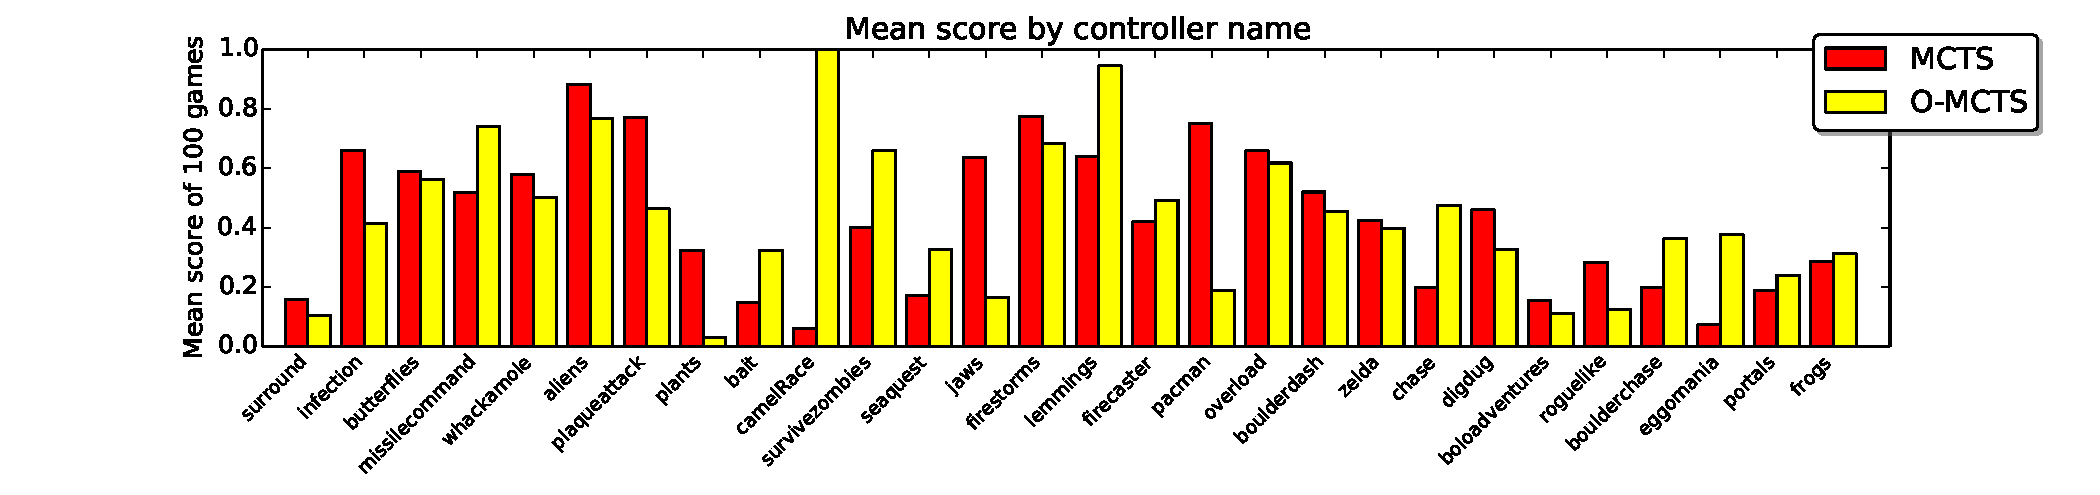
\includegraphics[width=\textwidth]{includes/scores}
\vspace{-.8cm}
\caption{Win ratio and mean normalized score of the algorithms per game. O-MCTS
outperforms MCTS in most games.}
\label{fig:scores}
\end{figure*}

In this section we describe our experiments on O-MCTS and OL-MCTS\@. The
algorithms are compared to the MCTS algorithm, as described in
Section~\ref{subsec:mcts}. All algorithms are run on a set of twenty-eight
different games in the VGDL framework. The set consists of all the games from
the first four training sets of the GVGAI competition, excluding puzzle games
that can be solved by an exhaustive search and have no random component (e.g.
NPCs). Each game has five levels.

Firstly, we compare O-MCTS to MCTS by showing the win ratio and mean score of
both algorithms on all the games. Secondly we show the improvement that OL-MCTS
makes compared to O-MCTS when it is allowed 4 games of learning time. 
%We demonstrate the progress it achieves by showing the first and last of the
%games it plays.  
Lastly we compare the three algorithms by summing up all the victories of all
the levels of each game.  
%Following the GVGAI competition's scoring method,
%algorithms are primarily judged on their ability to win the games. The scores
%they achieve are treated as a secondary objective.

For these experiments we construct an option set which is aimed at providing
action sequences for any type of game, since the aim here is general video game
playing.  Note that since the option set is a variable of the algorithm, either
a more specific or automatically generated set of options can be used by the
algorithm as well.

The set of option types consists of one option that executes a specific action
once, an option that avoids the nearest NPC by moving away from it, an option
that moves to a movable sprite until it is close to it (but not on it). There
are options that go to a movable sprite and options to go to a certain position
in the game.  Lastly we create an option that waits until an NPC is at a certain
distance and then fires the weapon.

For each option type, a subtype per visible sprite type is created during the
game. For each sprite, an option instance of its corresponding subtype is
created. For example, the game \textit{zelda} contains three different sprite
types (excluding the avatar and walls); monsters, a key and a portal. The first
level contains three monsters, one key and one portal. The aim of the game is to
collect the key and walk towards the portal without being killed by the
monsters. The score is increased by 1 if a monster is killed, i.e., its sprite
is on the same location as the sword sprite, if the key is picked up, or when
the game is won.  \emph{go to movable} and \emph{go near movable} options are
created for each of the three monsters and for the key. A \emph{go to position}
option is created for the portal.  One \emph{go to nearest sprite of type}
option is created per sprite type. One \emph{wait and shoot} option is created
for the monsters and one \emph{avoid nearest NPC} option is created. This set of
options is $O$, as defined in Section~\ref{subsec:options}. In a state where,
for example, all the monsters are dead, the possible option set $\mathbf{p}_s$
does not contain the \emph{avoid nearest NPC}, \emph{go to movable} and \emph{go
near movable} options for the monsters.

The \emph{go to \ldots} and \emph{go near \ldots} options utilize an adaptation
of the $A^*$ algorithm to plan their routes~\cite{hart1968formal}. An
adaptation is needed, because at the beginning of the game there is no knowledge
of which sprites are traversable by the avatar and which are not. Therefore,
during every move that is simulated by the agent, the $A^*$ module has to
update its beliefs about the location of walls and other blocking objects. This
is accomplished by comparing the movement the avatar wanted to make to the
movement that was actually made in game. If the avatar did not move, it is
assumed that all the sprites on the location the avatar should have arrived in
are blocking sprites. Our $A^*$ keeps a \emph{wall score} for each sprite type.
When a sprite blocks the avatar, its wall score is increased by one.
Additionally, to prevent the avatar from walking into deadly sprites, when a
sprite kills the avatar, its wall score is increased by 100.  Traditionally the
$A^*$'s heuristic uses the distance between two points. Our $A^*$ adaptation
adds the wall score of the goal location to this heuristic, encouraging the
algorithm to take paths with a low wall score. This method enables $A^*$ to
try to traverse paths that were unavailable earlier, while preferring safe and
easily traversable paths. For example in \textit{zelda}, a door is closed until
a key is picked up. Our $A^*$ implementation will still be able to plan a path
to the door once the key is picked up, to win the game.

We empirically optimize the parameters of the algorithms for these experiments.
We use discount factor $\gamma = 0.9$, maximum action time $t = 40$
milliseconds. The maximum search depth $d$ is set to 70, which is higher than
most alternative tree search algorithms, for example in the GVGAI competition,
use. This is possible because the search tree has a relatively low branching
factor. The number of node visits after which \textsf{uct} is used, $v$, is set
to 40. Crazy stone parameter $K$ is set to $0.5$.  For comparison, we use the
MCTS algorithm provided with the Java implementation of VGDL which employs a
maximum tree depth of 10, because the branching factor is higher. Both
algorithms have \textsf{uct} constant $C_p = \sqrt{2}$. Unfortunately, comparing
to Q-learning with options was impossible, because the state space of these
games is too big for the algorithm to learn any reasonable behavior. All the
experiments are run on an Intel i7--2600, 3.40GHz quad core processor with 6 GB
of DDR3, 1333 MHz RAM memory. In all the following experiments on this game set,
each algorithm plays each of the 5 levels of every game 20 times.

%\subsection{O-MCTS}
%\label{subsec:omcts}
First, we will describe the results of the O-MCTS algorithm in comparison with
MCTS\@.  This demonstrates the improvement that can be achieved by using our
algorithm.  The games in this and the following
experiments are ordered from left to right by the performance of an algorithm
that always chooses a random action, indicating the complexity of the games.
Figure~\ref{fig:scores} shows the win ratio and normalized score of the
algorithms for each game. In short, the O-MCTS algorithms performs at least as
good as MCTS in almost all games, and better in most.

O-MCTS outperforms MCTS in the games \textit{missile command}, \textit{bait},
\textit{camel race}, \textit{survive zombies}, \textit{firestorms},
\textit{lemmings}, \textit{firecaster}, \textit{overload}, \textit{zelda},
\textit{chase}, \textit{boulderchase} and \textit{eggomania} winning more games
or achieving a higher mean score. By looking at the algorithm's actions for
these games, we can see that O-MCTS succeeds in efficiently planning paths in a
dangerous environment, enabling it to do a further forward search than MCTS\@. 
\textit{Camel race} requires the player to
move to the right for 80 consecutive turns to reach the finish line. No
intermediate rewards are given to indicate that the agent is walking in the
right direction. This is hard for MCTS, since it only looks 10 turns ahead.
O-MCTS always wins this game, since it can plan forward a lot further.
Furthermore, the rollouts of the option for walking towards the finish line have
a bigger chance of reaching the finish line than the random rollouts executed by
MCTS\@.
In \textit{Overload}, a sword has to be picked up before the avatar can finish the
game, which seems to be too hard for MCTS, but poses less of a problem for
O-MCTS\@.  Furthermore, in \textit{zelda} we can see that the MCTS algorithm
achieves roughly the same score as O-MCTS, but does not win the game, since
picking up the key and walking towards the door is a difficult action sequence.
We assume that the mean score achieved by MCTS is because it succeeds in killing
the monsters, whereas O-MCTS achieves its score by picking up the key and
walking to the door.  These results indicate that O-MCTS performs better than
MCTS in games where a sequence subgoals have to be reached.

The MCTS algorithm performs better than O-MCTS in \textit{pacman},
\textit{whackamole}, \textit{jaws}, \textit{seaquest} and \textit{plaque attack}
(note that for \textit{seaquest}, O-MCTS has a higher mean score, but wins less
than MCTS). A parallel between these games is that they have a very
big number of different sprites, for each of which several options have to be
created by O-MCTS\@. When the number of options becomes too big, constructing the
set of possible options $\mathbf{p}_s$ for every state $s$ becomes so
time-consuming that the algorithm has too little time to build a tree and find
the best possible action. To test this hypothesis we increased the computation
time for O-MCTS to 120ms and found that the win ratio of O-MCTS increases to
around $0.8$ for \textit{seaquest} and \textit{plaque attack}, whereas the win
ratio for MCTS increased to $0.9$ and $0.7$ respectively. This means that with
more action time, the difference between O-MCTS and MCTS is reduced for
\textit{seaquest} and O-MCTS outperforms MCTS on \textit{plaque attack}.

\begin{figure}
	\centering
	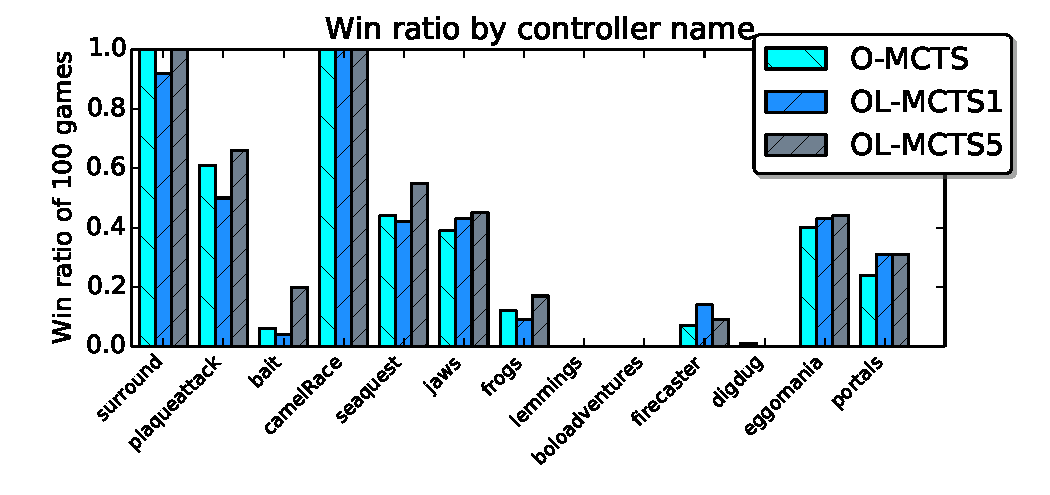
\includegraphics[width=\columnwidth]{includes/winsOLMCTS}
	%\vspace{-.8cm}
	%\caption{Win ratio comparison of OL-MCTS and O-MCTS.}
	%\label{fig:wins-olmcts}
	\centering
	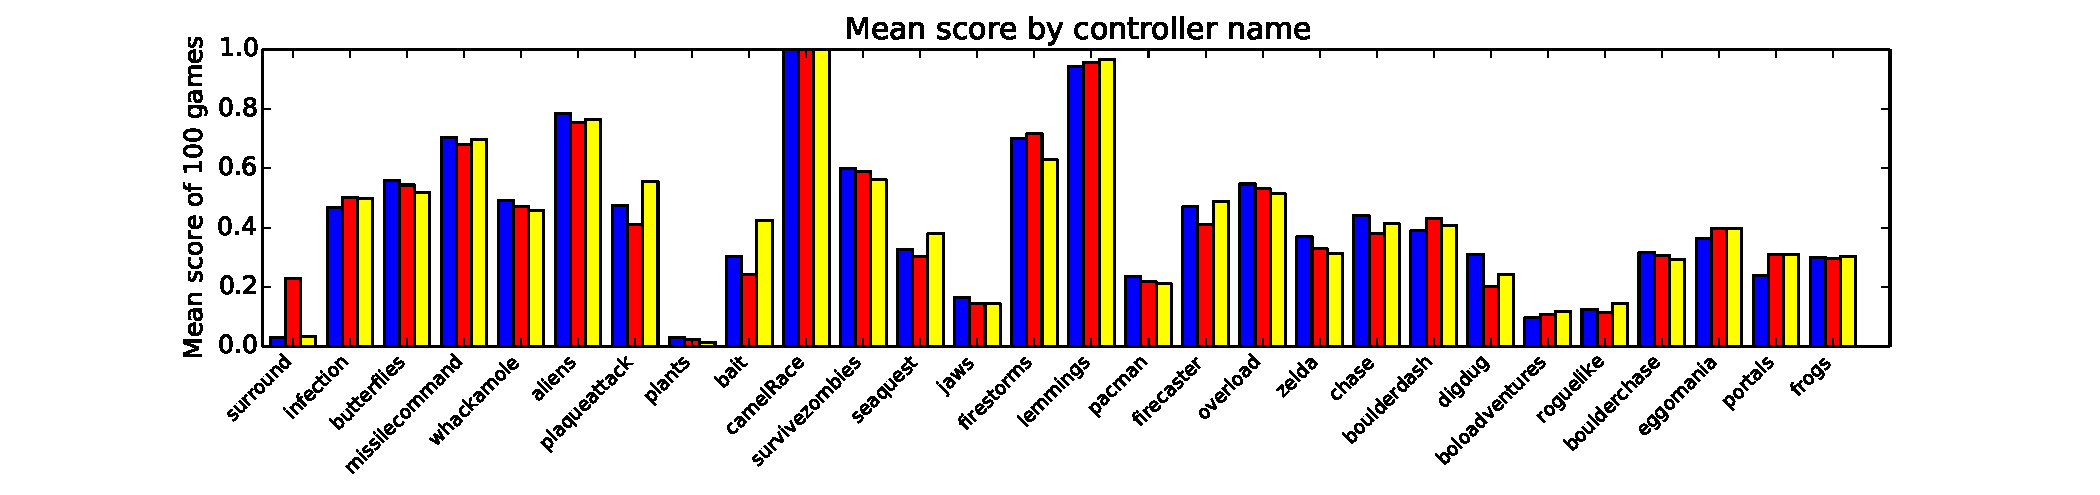
\includegraphics[width=\columnwidth]{includes/scoresOLMCTS}
	\vspace{-.8cm}
	\caption{Normalized win ratio and score comparison of OL-MCTS and O-MCTS\@.
	OL-MCTS outperforms O-MCTS by a small margin in some games. In the games
	that are not shown both algorithms perform equally.}
\label{fig:scores-olmcts}
\end{figure}

%\subsection{OL-MCTS}
%\label{subsec:olmcts}
Secondly, we compare OL-MCTS to O-MCTS by running it on the same set of games.
The option learning algorithm is allowed four learning games, after which the
fifth is used for the comparisons. Figure~\ref{fig:scores-olmcts} shows the
performance difference between O-MCTS and OL-MCTS on some games. For the other
games, the performance was approximately the same. Here OL-MCTS1 shows the
performance of OL-MCTS on the first game. OL-MCTS5 shows the performance of the
algorithm after learning for four games. 

We can see that, although the first iteration of OL-MCTS sometimes performs a
bit worse than O-MCTS, the fifth iteration often scores at least as high, or
higher than O-MCTS\@. We expect that the loss of performance in OL-MCTS1 is
a result of the extra overhead that is added by the crazy stone algorithm: a
sorting of all the option values has to take place in each tree node. The
learning algorithm significantly improves score and win ratio for the game
\textit{bait}.
%, which is a game in which the objective is to reach a goal portal
%after collecting a key.  The player can push boxes around to open paths. There
%are holes in the ground that kill the player unless they are filled with boxes,
%which make both the hole and the box disappear.
Figure~\ref{fig:learning-results} shows the improvement in score and win ratio
for this game. There are two likely explanations for this improvement: 1. There
are sprites that kill the player, which are evaded by the algorithm when it has
learned to do so.  2. The algorithm learns that it should pick up the key.

Furthermore, we can see small improvements on the games \textit{seaquest} and
\textit{jaws}, on which O-MCTS performs worse than MCTS\@.  Although OL-MCTS
does not exceed the score of the MCTS algorithm, this improvement suggests
that OL-MCTS is on the right path of improving O-MCTS\@.

\begin{figure}
	\centering
	\subfigure[Learning \textit{bait}]{%
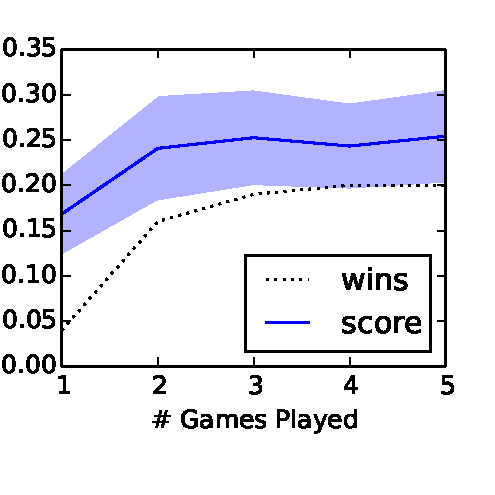
\includegraphics[scale=.44]{includes/learning}%
\label{fig:learning-results}%
	}
	\subfigure[Totals]{%
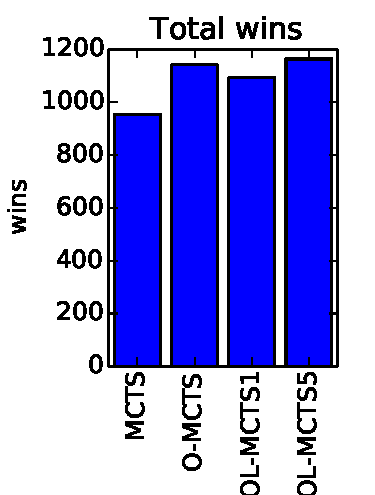
\includegraphics[scale=.44]{includes/totals.pdf}%
\label{fig:total-results}%
	}
	\caption{Learning improvement on game \textit{bait}, it shows win ratio and
		normalized score. Total number of wins of the algorithms on
	all games.}
\end{figure}

\subsection{Results}
\label{subsec:totals}
Summarizing, our tests indicate that on complex games O-MCTS outperforms MCTS\@.
For other games it performs at least as well, as long as the number of game
sprites is not too high.  The OL-MCTS algorithm can increase performance for
some of the games, such as \textit{bait} and \textit{plaque attack}. On other
games, little to no increased performance can be found.

An overview of the results is depicted in Figure~\ref{fig:total-results}, which
shows the sum of wins over all games, all levels.  It shows a significant ($p <
0.05$) improvement of O-MCTS and OL-MCTS over MCTS\@.  There is no significant
difference between performance of OL-MCTS over O-MCTS, although our results
suggest that it does improve for a subset of the games.


\section{Related Work}
\label{sec:related}
This section will cover some popular alternatives to O-MCTS and explain the
differences. \emph{Deep Q networks (DQN)} is a popular algorithm that trains a
convolutional neural network for a game \cite{mnih2013playing}, \emph{Planning
under Uncertainty with Macro-Actions (PUMA)} is a forward search algorithm that
uses extended actions in \emph{partially observable MDPs (POMDPs)}
\cite{he2010puma}.  \emph{Purofvio} is an algorithm that combines MCTS with
macro-actions that consist of repeating one action several times
\cite{powley2012monte}.

DQN trains a convolutional neural network that has the last four frames of a
game as input and tries to predict the Q-values of each action. A good policy
can then be created by selecting the action with the highest Q-value. The main
difference between O-MCTS and DQN is that O-MCTS has to select an optimal action
after 40 milliseconds, even when playing an unknown game. DQN learns for several
days, after which a good policy can be learned.  Furthermore, DQN does not use a
forward model, but always applies actions directly to the game in order to
learn.  Therefore, no accurate comparison can be made.

Another alternative is the PUMA algorithm, which applies forward search to
options (referred to as macro-actions) and works on POMDPs. The key difference
between PUMA and O-MCTS is that PUMA automatically generates goal-oriented MDPs
for specific subgoals. The advantage of which is that effective options can be
created without requiring any prior knowledge of the (PO)MDP. The disadvantage
is that this takes a lot of computation time and thus would not work in the
GVGAI framework, where only 40 milliseconds of computing time is allowed between
actions. Furthermore PUMA has to find out the optimal length per macro-action,
whereas O-MCTS can use options of variable length with starting an stopping
conditions.

A last alternative to O-MCTS is MCTS with macro actions called Purofvio.
Similar to O-MCTS, Purofvio plans over macro-actions, which are defined as
repeating an action several times. No more complex options are defined. The
paper notes that their options must always be of the same size, because they
found that otherwise MCTS seems to favor options with a longer time span over
shorter options. This problem does not exist in O-MCTS, probably because we
discount the option values. Furthermore Purofvio is only created for the
physical travelling salesperson problem, whereas O-MCTS can be used on many
different games. It must be noted though, that Purofvio could also work on other
games.


\section{Conclusions and Future Work}
\label{sec:conclusion}
We can conclude that the Option MCTS algorithm almost always performs at least
as good as MCTS. The O-MCTS algorithm excels in games with both a small level
grid or a small amount of sprites and high complexity, such as \textit{zelda},
\textit{overload} and \textit{eggomania}.  Furthermore, O-MCTS can look further
ahead than most tree searching alternatives, resulting in a high performance on
games like \textit{camel race}, in which reinforcement is sparse. This confirms
our hypothesis that using options, O-MCTS can win more games than MCTS. The
algorithm performs worse than expected in games with a high amount of sprites,
since the size of the option set becomes so large that maintaining it takes a
lot of time, leaving too little time for tree building. Over all twenty-eight
games, O-MCTS wins more games than MCTS.

The results of OL-MCTS indicate that it is possible to learn about which options
work better, meaning that in the future it should be possible to completely
remove infeasible options that have low expected rewards from the option set. We
expect that this could reduce the computation time O-MCTS needs to construct and
check all the options. However, more work needs to be done in this area to
enable improvement.

Furthermore, more research should be done in the influence of the option set.
Currently the effectiveness of the algorithm strongly relies on the A Star
implementation. This implementation is too time consuming, leaving
little time for actual tree building. In future work, trials can be done with
simpler and computationally cheaper alternatives, such as for example Enforced
Hill Climbing, as proposed in \cite{ross2014general}, although that has the
problem that the agent can get stuck. Alternatively, by creating goal-oriented
MDPs similar to PUMA's, the algorithm could probably increase sturdiness.

In order to improve the learning algorithms, some other improvements can be
investigated. Firstly, the backup method can be tweaked. In
\cite{coulom2007efficient}, instead of the mean value other values like the
maximum return are used in the backup phase. This has a positive effect on the
action (or in our case option) choices, resulting in a better performance.
Furthermore, the mean and standard deviation of option returns are now
calculated over all the games, without regarding how long ago this game was
played. This might lead to underrated options, for example with doors that
unlock under specific conditions (for example when the key is picked up in
\textit{zelda}).  Using a maximum return or discounting the option values might
have a different effect.



\bibliographystyle{abbrv}
\bibliography{bib}  % sigproc.bib is the name of the Bibliography in this case
% You must have a proper ".bib" file
%  and remember to run:
% latex bibtex latex latex
% to resolve all references
%
% ACM needs 'a single self-contained file'!
%
%APPENDICES are optional
%\balancecolumns
%\appendix
%Appendix A
%\balancecolumns % GM June 2007
% That's all folks!
\end{document}
